
\chapter{Revision and consolidation}
\section{Revision strategy}
\begin{retenir}
Effective revision alternates retrieval from memory, explicit correction of mistakes and reuse in a problem. Passively rereading the course is not enough: you must attempt a question without a model, compare your answer, then redo the question after a delay.
\end{retenir}

For each chapter, use the following code: \textbf{V} (mastered), \textbf{O} (shaky), \textbf{R} (to redo). After the diagnosis, work first on an orange or red skill, then check immediately with a similar question.

\begin{center}
\begin{tabularx}{.9\textwidth}{lcccX}
\toprule
Skill & V & O & R & Remedial action \\
\midrule
Choosing a model & $\square$ & $\square$ & $\square$ & Redo a sorting exercise: arithmetic/geometric/exponential.\\
Reading and calculating & $\square$ & $\square$ & $\square$ & Redo the targeted fluency exercises.\\
Writing up and interpreting & $\square$ & $\square$ & $\square$ & Add data, formula, calculation, unit and concluding sentence.\\
\bottomrule
\end{tabularx}
\end{center}

\sessionheader{52}{11 May 2027}{B: 2 h -- C: 1 h}{Diagnosis of what has been learned}{Revision and consolidation}
\begin{objectifs}\begin{itemize}\item Identify what has been learned.\item Classify the mistakes.\item Plan the remediation.\end{itemize}\end{objectifs}
\begin{automatismes}\begin{enumerate}\item Write the multiplier for an increase of $25\,\%$. \rep{$1+\dfrac{25}{100}=1.25$}\item Give the formula for the general term of an arithmetic sequence starting from $u_0$. \rep{$u_n=u_0+nr$}\item Solve $10^x=1000$. \rep{$x=3$}\item Differentiate $x+\dfrac4x$. \rep{$1-\dfrac4{x^2}$}\item State the law of total probability with two branches. \rep{$P(B)=P(A)P_A(B)+P(\overline A)P_{\overline A}(B)$}\end{enumerate}\end{automatismes}
\begin{prerequis}Reread the last written record and be able to carry out the basic calculations needed today. Before the investigation, have students rephrase the key words: identify what has been learned and classify the mistakes.\end{prerequis}

\begin{activite}
Answer 14 questions without the course, two per chapter. Record each mistake in a grid: knowledge, choice of method, calculation, reading, write-up. Then choose two personal priorities.

\end{activite}
\enseignant{The correction expects a profile of mistakes and a plan for catching up, not just an overall mark. Have students say aloud which piece of data triggers the choice of method.}

\begin{traceecrite}The diagnosis is used to choose the remediation: recognise the mistake, recall the useful rule, redo a similar question, then check without help.\end{traceecrite}

\begin{exemple}
Take the data from the investigation and write the solution in order: definition of the objects, property used, exact or approximate calculation, then a concluding sentence. The model answer is in the teacher edition.
\end{exemple}
\enseignant{The correction expects a profile of mistakes and a plan for catching up, not just an overall mark.}

\begin{exercice}[-- essential]
\begin{enumerate}\item Choose between an arithmetic sequence, a geometric sequence and an exponential function in three situations.\item Solve an exponential equation using a logarithm.\item Calculate a probability from a tree, then interpret it.\end{enumerate}
\end{exercice}
\enseignant{Justify each choice by absolute or relative change; check positivity before taking the logarithm; multiply along a path and conclude with a sentence.}

\manuelref{Reactivation of chapters 1 to 7}
\ExoSession{52}

\begin{dm}Redo practice exercise 3 with the following data: replace the initial value by $380$ and the rate or common ratio by $6$. Write it up in four lines: data, formula, calculation, conclusion.\end{dm}
\enseignant{The solution depends on the exercise redone. Check above all the consistency of the model, the number of iterations, the rounding and the concluding sentence.}

\begin{sortie}On a half-sheet: write the main rule of the session, work through a very short example and give a confidence level from 1 to 4. Essential question(s) of the day: 1 and 2.\end{sortie}

\ifprof
\begin{methode}
\textbf{1 h session:} 7 min of fluency; 10 min of pooling and written record; 28 min of essential exercises; 5 min of correction; 3 min of exit ticket.\\
\textbf{2 h session:} add 20 min of investigation, 20 min of formalisation, a second independent exercise and 10 min of comparative correction.\\
\textbf{Differentiation:} give struggling students a four-box sheet (data, model, calculation, conclusion). Ask quick students to produce a counterexample, a justification or a second method.
\end{methode}
\fi
\sessionheader{53}{13 May 2027}{B: 1 h -- C: 2 h}{Reactivation: exponential functions}{Revision and consolidation}
\begin{objectifs}\begin{itemize}\item Reactivate exponential models.\item Solve and interpret.\item Check the units.\end{itemize}\end{objectifs}
\begin{automatismes}\begin{enumerate}\item Simplify $3x+7-x+2$. \rep{$2x+9$}\item Solve $10^x=1000$. \rep{$x=3$}\item Differentiate $x+\dfrac4x$. \rep{$1-\dfrac4{x^2}$}\item State the law of total probability with two branches. \rep{$P(B)=P(A)P_A(B)+P(\overline A)P_{\overline A}(B)$}\item Give the formula for the general term of an arithmetic sequence starting from $u_0$. \rep{$u_n=u_0+nr$}\end{enumerate}\end{automatismes}
\begin{prerequis}Reread the last written record and be able to carry out the basic calculations needed today. Before the investigation, have students rephrase the key words: reactivate exponential models and solve and interpret.\end{prerequis}

\begin{activite}
A value of $18\,000$ increases by $3.5\,\%$ per year. Write the model, calculate the value after eight years and determine when it will exceed $25\,000$.
\begin{center}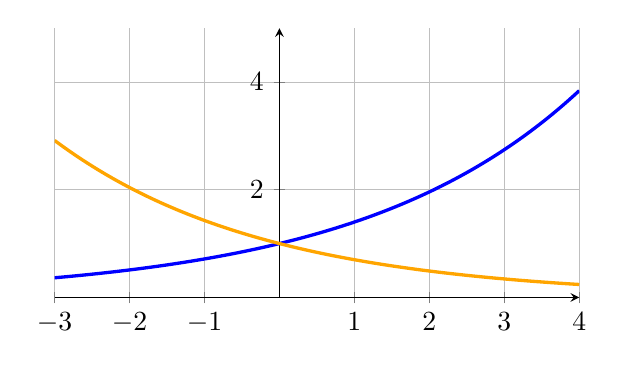
\begin{tikzpicture}\begin{axis}[width=.68\textwidth,height=5cm,axis lines=middle,xmin=-3,xmax=4,ymin=0,ymax=5,grid=major]\addplot[Blue,very thick,samples=100,domain=-3:4]{1.4^x};\addplot[Orange,very thick,samples=100,domain=-3:4]{.7^x};\end{axis}\end{tikzpicture}\end{center}
\end{activite}
\enseignant{$V(t)=18\,000\times1.035^t$, $V(8)\approx23\,703$. The threshold is exceeded from the tenth year onwards. Have students say aloud which piece of data triggers the choice of method.}

\begin{traceecrite}An exponential function models a constant relative change. First identify the initial value and the multiplier.\end{traceecrite}

\begin{exemple}
Take the data from the investigation and write the solution in order: definition of the objects, property used, exact or approximate calculation, then a concluding sentence. The model answer is in the teacher edition.
\end{exemple}
\enseignant{$V(t)=18\,000\times1.035^t$, $V(8)\approx23\,703$. The threshold is exceeded from the tenth year onwards.}

\begin{exercice}[-- essential]
\begin{enumerate}\item Choose between an arithmetic sequence, a geometric sequence and an exponential function in three situations.\item Solve an exponential equation using a logarithm.\item Calculate a probability from a tree, then interpret it.\end{enumerate}
\end{exercice}
\enseignant{Justify each choice by absolute or relative change; check positivity before taking the logarithm; multiply along a path and conclude with a sentence.}

\manuelref{Calao, p. 48, no.~1--8, then p. 54, no.~47--50}
\ExoSession{53}

\begin{dm}Redo practice exercise 2 with the following data: replace the initial value by $385$ and the rate or common ratio by $7$. Write it up in four lines: data, formula, calculation, conclusion.\end{dm}
\enseignant{The solution depends on the exercise redone. Check above all the consistency of the model, the number of iterations, the rounding and the concluding sentence.}

\begin{sortie}On a half-sheet: write the main rule of the session, work through a very short example and give a confidence level from 1 to 4. Essential question(s) of the day: 1, 2 and 3.\end{sortie}

\ifprof
\begin{methode}
\textbf{1 h session:} 7 min of fluency; 10 min of pooling and written record; 28 min of essential exercises; 5 min of correction; 3 min of exit ticket.\\
\textbf{2 h session:} add 20 min of investigation, 20 min of formalisation, a second independent exercise and 10 min of comparative correction.\\
\textbf{Differentiation:} give struggling students a four-box sheet (data, model, calculation, conclusion). Ask quick students to produce a counterexample, a justification or a second method.
\end{methode}
\fi
\sessionheader{54}{18 May 2027}{B: 2 h -- C: 1 h}{Reactivation: common logarithm (base 10)}{Revision and consolidation}
\begin{objectifs}\begin{itemize}\item Reactivate logarithms.\item Solve an equation.\item Check the conditions.\end{itemize}\end{objectifs}
\begin{automatismes}\begin{enumerate}\item Calculate $5\,\%$ of $160$. \rep{$8$}\item Differentiate $x+\dfrac4x$. \rep{$1-\dfrac4{x^2}$}\item State the law of total probability with two branches. \rep{$P(B)=P(A)P_A(B)+P(\overline A)P_{\overline A}(B)$}\item Give the formula for the general term of an arithmetic sequence starting from $u_0$. \rep{$u_n=u_0+nr$}\item Solve $10^x=1000$. \rep{$x=3$}\end{enumerate}\end{automatismes}
\begin{prerequis}Reread the last written record and be able to carry out the basic calculations needed today. Before the investigation, have students rephrase the key words: reactivate logarithms and solve an equation.\end{prerequis}

\begin{activite}
Solve $10^x=340$, $1.06^n=2$ and $1.06^n\geq2$. For each answer, distinguish the real value, the approximate value and the minimum integer index.

\end{activite}
\enseignant{$x\approx2.5315$; $n\approx11.90$; for the integer threshold, $n=12$. Have students say aloud which piece of data triggers the choice of method.}

\begin{traceecrite}The logarithm turns an exponential equation into an equation in the exponent. Conditions: base positive and different from $1$, right-hand side positive.\end{traceecrite}

\begin{exemple}
Take the data from the investigation and write the solution in order: definition of the objects, property used, exact or approximate calculation, then a concluding sentence. The model answer is in the teacher edition.
\end{exemple}
\enseignant{$x\approx2.5315$; $n\approx11.90$; for the integer threshold, $n=12$.}

\begin{exercice}[-- essential]
\begin{enumerate}\item Choose between an arithmetic sequence, a geometric sequence and an exponential function in three situations.\item Solve an exponential equation using a logarithm.\item Calculate a probability from a tree, then interpret it.\end{enumerate}
\end{exercice}
\enseignant{Justify each choice by absolute or relative change; check positivity before taking the logarithm; multiply along a path and conclude with a sentence.}

\manuelref{Calao, p. 70, no.~1--10, then pp. 73--75, no.~30--42}
\ExoSession{54}

\begin{dm}Redo practice exercise 3 with the following data: replace the initial value by $390$ and the rate or common ratio by $2$. Write it up in four lines: data, formula, calculation, conclusion.\end{dm}
\enseignant{The solution depends on the exercise redone. Check above all the consistency of the model, the number of iterations, the rounding and the concluding sentence.}

\begin{sortie}On a half-sheet: write the main rule of the session, work through a very short example and give a confidence level from 1 to 4. Essential question(s) of the day: 1 and 2.\end{sortie}

\ifprof
\begin{methode}
\textbf{1 h session:} 7 min of fluency; 10 min of pooling and written record; 28 min of essential exercises; 5 min of correction; 3 min of exit ticket.\\
\textbf{2 h session:} add 20 min of investigation, 20 min of formalisation, a second independent exercise and 10 min of comparative correction.\\
\textbf{Differentiation:} give struggling students a four-box sheet (data, model, calculation, conclusion). Ask quick students to produce a counterexample, a justification or a second method.
\end{methode}
\fi
\sessionheader{55}{20 May 2027}{B: 1 h -- C: 2 h}{Reactivation: reciprocal function}{Revision and consolidation}
\begin{objectifs}\begin{itemize}\item Reactivate the reciprocal function.\item Carry out a study.\item Sketch and interpret.\end{itemize}\end{objectifs}
\begin{automatismes}\begin{enumerate}\item Write the multiplier for an increase of $10\,\%$. \rep{$1+\dfrac{10}{100}=1.10$}\item State the law of total probability with two branches. \rep{$P(B)=P(A)P_A(B)+P(\overline A)P_{\overline A}(B)$}\item Give the formula for the general term of an arithmetic sequence starting from $u_0$. \rep{$u_n=u_0+nr$}\item Solve $10^x=1000$. \rep{$x=3$}\item Differentiate $x+\dfrac4x$. \rep{$1-\dfrac4{x^2}$}\end{enumerate}\end{automatismes}
\begin{prerequis}Reread the last written record and be able to carry out the basic calculations needed today. Before the investigation, have students rephrase the key words: reactivate the reciprocal function and carry out a study.\end{prerequis}

\begin{activite}
Study $f(x)=x+\dfrac{16}{x}$ on $]0,+\infty[$ and interpret its minimum in an average-cost context. Produce the table of variations and a sketch.
\begin{center}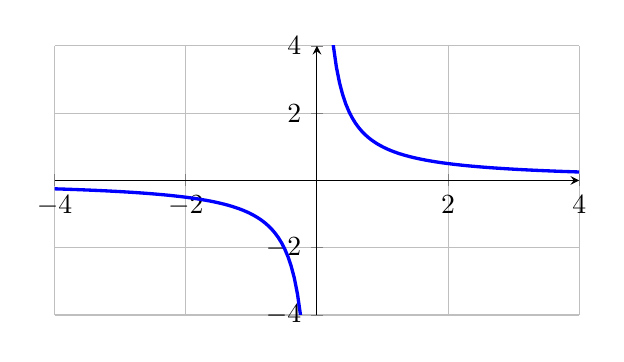
\begin{tikzpicture}\begin{axis}[width=.68\textwidth,height=5cm,axis lines=middle,xmin=-4,xmax=4,ymin=-4,ymax=4,grid=major]\addplot[Blue,very thick,samples=80,domain=-4:-.15]{1/x};\addplot[Blue,very thick,samples=80,domain=.15:4]{1/x};\end{axis}\end{tikzpicture}\end{center}
\end{activite}
\enseignant{$f'(x)=\dfrac{(x-4)(x+4)}{x^2}$; minimum $f(4)=8$. Have students say aloud which piece of data triggers the choice of method.}

\begin{traceecrite}For a function containing $\dfrac1x$, start by excluding $x=0$, then differentiate, factorise and study the sign before the variations.\end{traceecrite}

\begin{exemple}
Take the data from the investigation and write the solution in order: definition of the objects, property used, exact or approximate calculation, then a concluding sentence. The model answer is in the teacher edition.
\end{exemple}
\enseignant{$f'(x)=\dfrac{(x-4)(x+4)}{x^2}$; minimum $f(4)=8$.}

\begin{exercice}[-- essential]
\begin{enumerate}\item Choose between an arithmetic sequence, a geometric sequence and an exponential function in three situations.\item Solve an exponential equation using a logarithm.\item Calculate a probability from a tree, then interpret it.\end{enumerate}
\end{exercice}
\enseignant{Justify each choice by absolute or relative change; check positivity before taking the logarithm; multiply along a path and conclude with a sentence.}

\manuelref{Calao, p. 94, no.~1--9, then p. 96, no.~10--21}
\ExoSession{55}

\begin{dm}Redo practice exercise 2 with the following data: replace the initial value by $395$ and the rate or common ratio by $3$. Write it up in four lines: data, formula, calculation, conclusion.\end{dm}
\enseignant{The solution depends on the exercise redone. Check above all the consistency of the model, the number of iterations, the rounding and the concluding sentence.}

\begin{sortie}On a half-sheet: write the main rule of the session, work through a very short example and give a confidence level from 1 to 4. Essential question(s) of the day: 1, 2 and 3.\end{sortie}

\ifprof
\begin{methode}
\textbf{1 h session:} 7 min of fluency; 10 min of pooling and written record; 28 min of essential exercises; 5 min of correction; 3 min of exit ticket.\\
\textbf{2 h session:} add 20 min of investigation, 20 min of formalisation, a second independent exercise and 10 min of comparative correction.\\
\textbf{Differentiation:} give struggling students a four-box sheet (data, model, calculation, conclusion). Ask quick students to produce a counterexample, a justification or a second method.
\end{methode}
\fi
